%-------------------------------------------------------------------------------
% yum_menu
%-------------------------------------------------------------------------------
%
% \file        yum_menu.tex
% \library     Documents
% \author      Chris Ahlstrom
% \date        2017-09-24
% \update      2017-09-24
% \version     $Revision$
% \license     $XPC_GPL_LICENSE$
%
%     Provides the Scales section of yoshimi-user-manual.tex.
%
%-------------------------------------------------------------------------------

\section{Scales}
\label{sec:Scales}

   \textsl{Yoshimi} is a microtonal synthesizer, and is capable of a wide
   range of microtonal scales.  Many improvements have been made to the scales,
   including the user-interface, performance, accuracy of calculations,
   and adherence to the Scala (\cite{scala}) specification.
   in version 1.5.2 and above. At the request of users, since version 1.5.8 some controls have been made accessible to MIDI-learn, and these have the familiar pale blue border.
   \index{LV2!scales}
   For users of the LV2 plugin, any changes in scale
   settings are reported back so that the plugin host can be aware of the
   change.

\subsection{Scales / Command Line}
\label{subsec:scales_command_line}

	One can now fully control scales from the CLI.
	For tunings, either ratios or floating point numbers can be entered.
	Ratios are in the form
	\texttt{n1/n2} to a maximum of normal integer range.
   If just a numerator is set, it will be regarded as \texttt{n/1}.
   Floating point numbers \textsl{must}
   include the decimal point and at least one digit (or zero) on either side.
   The numbers are padded out with leading and trailing zeros in the form
   \texttt{nnnn.nnnnnn}.

   \index{scales!non-sounding notes}
   In keyboard maps, non-sounding notes should be entered as an 'x' instead of
   the key number.

   CLI tunings and keymaps are entered in CSV format.
   Tuning:

   \begin{verbatim}
      0076.049000, 0193.156860, 0310.264710, 5/4, 0503.421570,
      0579.470570, 0696.578430, 25/16, 0889.735290, 1006.843140,
      1082.892140, 2/1
   \end{verbatim}

   Keymap:

   \begin{verbatim}
      0, 1, 2, 3, x, 5, 6, 7, x, 9, 10, 11
   \end{verbatim}

   The tuning/keymap sizes are generated internally by counting the number of
   entries in the strings.

   When saving scales, for floating point numbers, \textsl{Yoshimi} includes
   the text it was derived from. This has accuracy benefits,
   but also reassures less experienced users,
   because the values they enter won't seem to change on
   re-loading.  The stored value is still saved for backward compatibility with
   older versions of \textsl{Yoshimi}.

   \index{scales!shift}
   Scale shift provides an offset to the scale start position, and only makes a
   difference in uneven interval sizes.

   Normally (for the even tempered scale) the scale starts on 'A', and, as the
   intervals are all identical, changing the octave start will make no
   difference. However, if one has (say) a 5-note pentatonic scale, the
   intervals will be very different and the scale shift will effectively
   determine the key of the scale.

\begin{figure}[H]
   \centering
   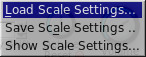
\includegraphics[scale=0.9]{menu/yoshimi-menu-scales.jpg}
   \caption{Yoshimi Menu, Scales}
   \label{fig:yoshimi_scales}
\end{figure}

   \begin{enumber}
      \item \textbf{Show Settings...}
      \item \textbf{Load...}
      \item \textbf{Save...}
      \item \textbf{Recent Scales...}
      \item \textbf{Clear}
   \end{enumber}

\subsection{Scales / Show Settings}
\label{subsec:scales_show}

\begin{figure}[H]
   \centering
   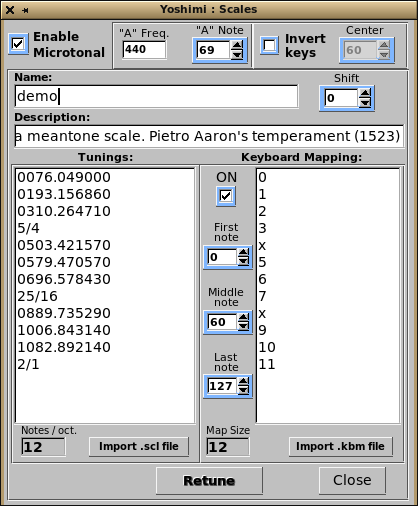
\includegraphics[scale=0.75]{1.6.0/Scales.png}
   \caption{Yoshimi Menu, Scales Settings}
   \label{fig:yoshimi_scales_settings}
\end{figure}

\subsubsection{Scales Basic Settings}
\label{subsubsec:scales_basic_settings}

   This item controls the microtonal capabilities of \textsl{Yoshimi} and
   some other settings related to tuning.
   The last entry in the tunings list represents one octave.
   All other notes are deduced from these settings.

   \begin{enumber}
      \item \textbf{Enable Microtonal}
      \item \textbf{(Ref.) Freq.}
      \item \textbf{(Ref.) Note}
      \item \textbf{Invert Keys}
      \item \textbf{Center}
      \item \textbf{Name}
      \item \textbf{Shift}
      \item \textbf{Comment}
      \item \textbf{Tunings}
      \item \textbf{Retune}
      \item \textbf{Keyboard Mapping}
      \item \textbf{ON}
      \item \textbf{First note}
      \item \textbf{Middle note}
      \item \textbf{Last note}
      \item \textbf{nts./oct.}
      \item \textbf{Import .scl file}
      \item \textbf{Map Size}
      \item \textbf{Import .kbm file}
      \item \textbf{Close}
   \end{enumber}

   \setcounter{ItemCounter}{0}      % Reset the ItemCounter for this list.

   \itempar{Enable Microtonal}{Enable Microtonal}
   Enable Microtonal Scales.
   When disabled, the synthesizer will use equal-temperament, 12 notes per
   octave.  Otherwise, one can input any scale one desires.
   In \textsl{Yoshimi} V 1.6.1 this was revised to more correctly identify
   the frequency and note settings. The ranges have also been reduced to
   reduce the risk of possible damage to audio equipment. They are still
   well outside any reasomable requirement.

   Values: \texttt{Off*, On}

   \itempar{(Ref.) Freq}{Frequency}
   Frequency of the reference note.
   Sets the frequency of the reference key. The standard is "A", 440.0 Hz.

   Values: \texttt{30 to 1100, 440*}

   \itempar{(Ref.) Note}{MIDI note number}
   Sets the MIDI value of the refencence note. This is usually number 69,
   which is A4

   Values: \texttt{24 to 84, 69*}

   \itempar{Invert Keys}{keys}
   Allows the keys to be inverted, so that higher-valued keys play lower
   notes.

   Values: \texttt{Off*, On}

   \itempar{Center}{center}
   Center for Inverted Keys.
   This is the center where the notes frequencies are turned upside-down if
   \textbf{Invert keys} is enabled.
   If the center is 60, the note 59 will become 61, 58 will become 62, 61
   will become 59, and so on.

   Values: \texttt{0 to 127, 60*}

   \itempar{Name}{mapping}
   Name of the Mapping.
   For example, the default mapping is called "12tET".

   \itempar{Shift}{key shift}
   Key Shift.
   Shift the scale. If the scale is tuned to A, one can easily tune it to
   another key.

   Values: \texttt{-63 to 64, 0*}

   \itempar{Comment}{comment}
   Comment for Key Mapping.
   Provides a comment or a description of the scale.
   By default, this is "Equal Temperament 12 notes per octave".

   \itempar{Tunings}{tuning}
   Tunings.
   Here one can input a scale by entering all the tunings for one octave.
One can enter the tunings in two ways:

   \begin{enumber}
      \item As the number of cents (1200 cents=1 octave) as a float number
         like "100.0", "123.234"
      \item As a proportion like "2/1" which represents one octave, "3/2" a
         perfect fifth, "5734/6561".  "2/1" is equal to "1200.0" cents.
   \end{enumber}

   The default is a series of values:
   \texttt{0100.0, 0200.0, ..., 1100.0, 2/1}.

   \itempar{Keyboard Mapping}{keyboard}
   The items related to the \textbf{Keyboard Mapping} are discussed
   separately in the next section.

   \itempar{Retune}{retune}
   Retune button.
   This button retunes the synthesizer according to the settings of
   the \textbf{Tunings} and \textbf{Keyboard Mapping} lists.
   The \textbf{Retune} button is needed if one
   changes any of the actual scale settings. However, it's not needed for key
   mappings or any other controls, all of which operate immediately.

   \itempar{Notes/oct}{Notes per Octave}
   Notes Per Octave.
   This value is affected by changes to the \textbf{Tunings} mapping.

   Values: \texttt{12*}

   \itempar{Import .SCL file}{scale file}
   Import Scala files.
   Scala is a powerful application for experimentation with musical tunings
   (intonation scales, micro-tonal,...etc.). From its home page \cite{scala},
   one can download more than 2800 scales which one can import directly into
   \textsl{Yoshimi}.  Note that the zip file \textsl{must} be unzipped with
   the \texttt{-aa} ("autoconvert") option.  However, we have converted it to a
   much smaller tar file (it crams 18 Mb of files into an sub-500 Kb file),
   which can be untarred directly into
   one's configuration directory to create a
   \texttt{\textasciitilde/.config/yoshimi/scales} directory chock full of
   scales.

    \begin{verbatim}
      $ cd ~/.config/yoshimi/
      $ tar xf yoshimi-scales.tar.xz
    \end{verbatim}

    Note that a Scala file cannot be loaded directly.  It must be imported.

\begin{figure}[H]
   \centering
   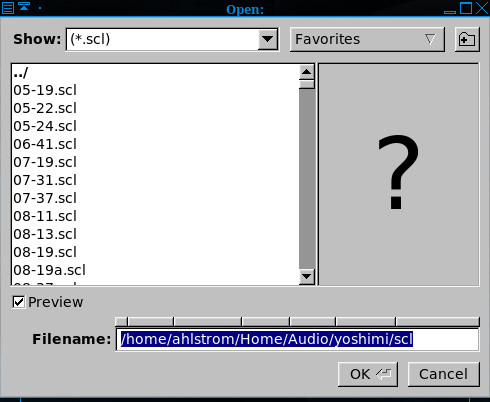
\includegraphics[scale=0.75]{menu/Scales/import-scl-file.jpg}
   \caption{Yoshimi Menu, Scales, Import File}
   \label{fig:yoshimi_scales_import_file}
\end{figure}

%  \itempar{Import .scl file}{scl file}
   This item is a standard file dialog for reading
   a \texttt{*.scl} file.

\begin{figure}[H]
   \centering
   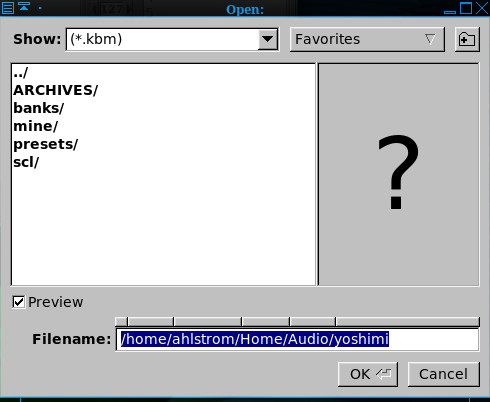
\includegraphics[scale=0.75]{menu/Scales/import-kbm-file.jpg}
   \caption{Yoshimi Menu, Scales, Import Keyboard Map}
   \label{fig:yoshimi_scales_import_keyboard_map}
\end{figure}

   \itempar{Map Size}{scales!map size}
   Map Size.
   This value is affected by changes to the \textbf{Keyboard Mapping}.

   Values: \texttt{12*}

   \itempar{Import .kbm file}{kbm file}
   This item is a standard file dialog for reading
   a \texttt{*.kbm} file.

   \itempar{Close, Scales Dialog}{close scales}

\subsubsection{Keyboard Mapping}
\label{subsubsec:scales_keyboard_mapping}

   One can set the MIDI keyboard mapping to scale-degree mapping.
   This is used if the scale has more or less than 12 notes/octave.
   One can enable the mapping by pressing the \textbf{ON} check-box.

   \begin{enumber}
      \item \textbf{ON}
      \item \textbf{First Note}
      \item \textbf{Last Note}
      \item \textbf{Middle Note}
      \item \textbf{Map}
      \item \textbf{Map Size}
   \end{enumber}

   \setcounter{ItemCounter}{0}      % Reset the ItemCounter for this list.

   \itempar{ON}{scales!on}
   This item enables the \textbf{Keyboard Mapping} list.

   Values: \texttt{Off*, On}

   \itempar{First Note}{scales!first note}
   First MIDI Note Number.
   Sets the MIDI note value to use for the first note of the scale.
   MIDI notes below this value are ignored.

   Values: \texttt{0* to 127}

   \itempar{Middle Note}{scales!middle note}
   Sets the MIDI note value to use for the middle note of the scale.
   This is the note where the scale-degree 0 setting is mapped;
   the middle note represents the note where the formal octave starts.

   Values: \texttt{0 to 127, 60*}

   \itempar{Last Note}{scales!last note}
   Last MIDI Note Number.
   Sets the MIDI note value to use for the last note of the scale.
   Keys above this value are ignored.

   Values: \texttt{0 to 127*}

   \itempar{Map}{scales!map}
   Scales map.  This is the input field where the mappings are entered.
   The numbers represent the order (degree) entered on
   \textbf{Tunings Input} field, with the first value being 0.
   This number must be less than the number of notes per octave (since
   the values start at 0).
   If one doesn't want a key to be mapped, one enters an "x" instead of a
   number.

   Values: \texttt{0 to 11}

   \itempar{Map Size}{scales!map size}
   Provides the size of the scale-map.

   Values: \texttt{12}

   In the current version of \textsl{Yoshimi}, up to 25 recently used scales are
   now stored in the new history file
   (\texttt{yoshimi.history}), and can be quickly reinstalled with a
   mini-browser in exactly the same way as patch sets.

\subsection{Scales / Load}
\label{subsec:scales_load}

\begin{figure}[H]
   \centering
   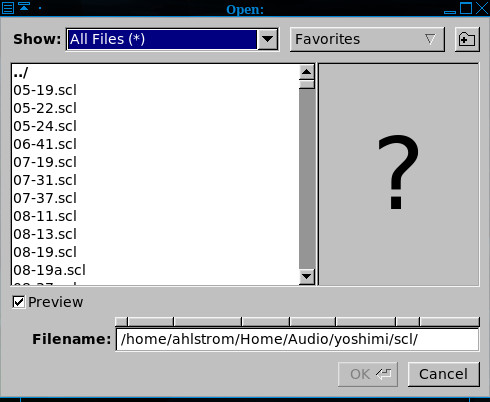
\includegraphics[scale=0.75]{menu/Scales/open-scales.jpg}
   \caption{Yoshimi Menu, Open Scales}
   \label{fig:yoshimi_open_scales}
\end{figure}

   If the format of the scales file is not correct, then the following prompt
   will appear.

\begin{figure}[H]
   \centering
   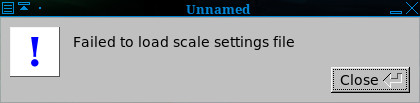
\includegraphics[scale=0.75]{menu/Scales/failed-to-load-scl-file-vice-xsz.jpg}
   \caption{Yoshimi Menu, Failed to Load Scales}
   \label{fig:yoshimi_failed_to_load_scales}
\end{figure}

   Note that the loading and saving of scales is fully available in the
   command-line as well.

\subsection{Scales / Save}
\label{subsec:scales_save}

   This dialog opens a stock file-dialog to allow the saving of
   \texttt{*.xsz} files.
   If one has imported a scale from an \texttt{*.scl} file, and one
   wants direct access to it from the \textbf{Scales / Recent Scales} menu, one
   must first save the imported file as an \texttt{*.xsz} files.

   Note that the loading and saving of scales is fully available in the
   command-line as well.

   In the past, every time one saved and reloaded a scale, there was a
   degradation in the accuracy of the scales.  This issue has been fixed, since
   people are very sensitive to pitch intervals.

\subsection{Scales / Recent Scales...}
\label{subsec:scales_recent_scales}

   Once a scale file has been loaded (or imported and saved), then it
   becomes available in this list, for more convenient access to it.

\begin{figure}[H]
   \centering
   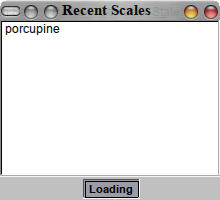
\includegraphics[scale=0.75]{menu/Scales/recent-scales.png}
   \caption{Yoshimi Menu, Recent Scales}
   \label{fig:yoshimi_recent_scales}
\end{figure}

\subsection{Scales / Clear}
\label{subsec:scales_clear}

   This menu entry simply resets the \textsl{Yoshimi} scale back to it default,
   the twelve-tone equally-tempered scale.

\subsection{Scales / Reference Pitch...}
\label{subsec:scales_reference_pitch}
   A note about relationships between the reference note frequency, note number
   and key shifts.

   The reference note frequency should be regarded as an absolute value, with the
   note number being specifically a MIDI representation.
   Master keyshift, and Part keyshifts are relative values that modify this for
   convenience.

   As an example, some very old wood-framed pianos were tuned with C4=256 cycles
   per second (Hz). This can't be changed as the frame couldn't withstand the
   extra stress, so to play alongside such a piano one would have to set the
   absolute value 'A' frequency at 430.581Hz. Better still would be to set note
   number 60 to a frequency of 256! If you have the reports window open you will see the following responses, making it quite clear what has changed.

   \begin{verbatim}
      Scales Ref note 60 (C4)
      Scales (C4) Frequency Value 256.000000
   \end{verbatim}

   A singer might then say they couldn't sing at that pitch, so one would then use
   the Master Keyshift to change to a key they were more comfortable with.

   When playing \textsl{Yoshimi} in a band where there is a minor pitch
   discreapancy it would be best to use the Master Detune to match, rather than
   altering the reference frequency.

   Since V 1.5.11 reference frequency range has been limited, and revised further
   since V 1.6. The range is 30Hz to 1100Hz which covers
   the range B0 to C6. Previously it could be set anywhere between 1Hz and 2000Hz.
   Not only did this put most notes right out of the audio spectrum, but it was
   potentially damaging for some audio equipment.

   With the various key shift and octave controls it is still possible to cover
   every part of the audio spectrum.

%-------------------------------------------------------------------------------
% vim: ts=3 sw=3 et ft=tex
%-------------------------------------------------------------------------------
